% PROGETTAZIONE E CODIFICA

\chapter{Progettazione e codifica}\label{chap:design}

\section {Progettazione architetturale}

\section{Progettazione grafica}
Prima di procedere alla definizione delle classi necessarie per l'implementazione dell'applicazione è stato deciso di effettuare un lavoro di progettazione grafica per far si che il progetto di stage abbracciasse a 360 gradi il processo di sviluppo di un'applicazione da parte di un'azienda.
\subsection{Wireframe}
In base ai requisiti e agli use case raccolti è stato definito il modello iniziale di rappresentazione dell'applicazione tramite la realizzazione dei wireframe delle varie schermate. \\
Questo studio è la prima rappresentazione visuale dell'applicazione ed ha lo scopo di identificare la struttura, l'architettura dell'informazione e la disposizione degli elementi nella pagina.\\
Di seguito vengono riportati i wireframe di alcune delle pagine più importanti di Teamwork:

\begin{figure}[H] 
	\centering
	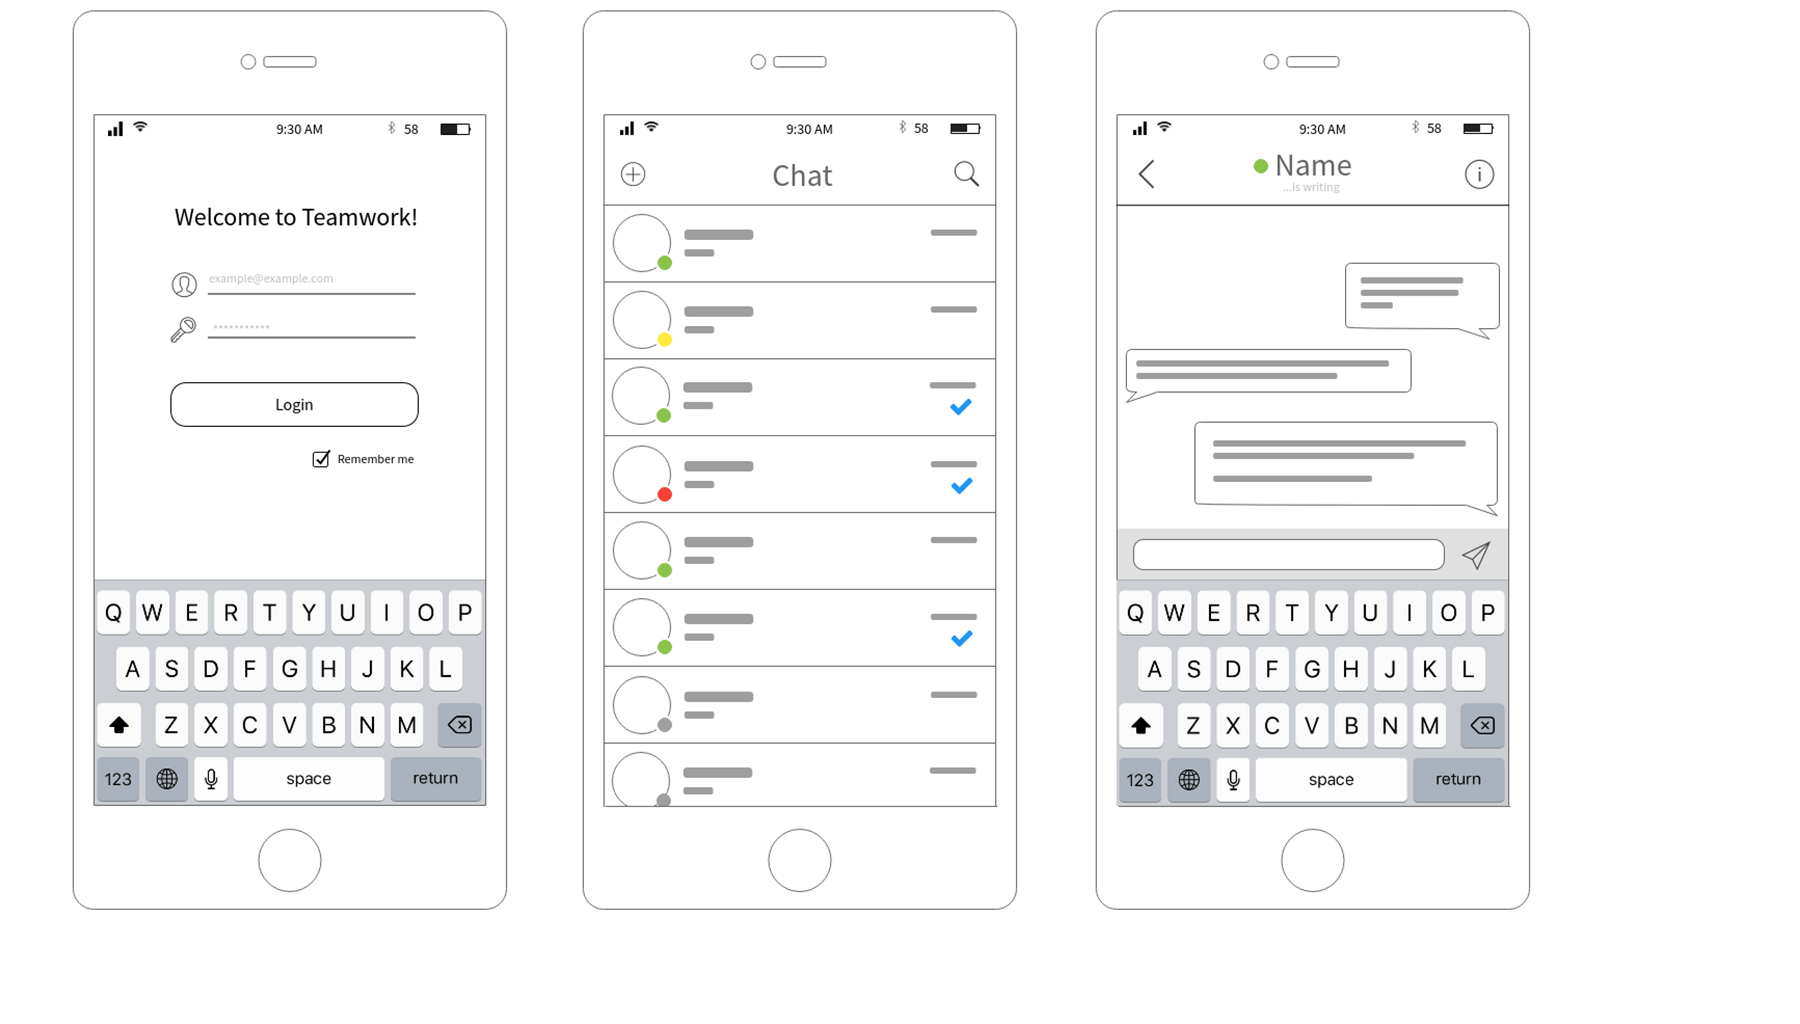
\includegraphics[scale=0.5]{wireframe}
	\caption{UCG - Caso d'uso generale}
\end{figure}


\section{Progettazione di dettaglio}
Approvati questi wireframe è stato potuto proseguire alla definizione di tutti e soli i componenti veramente utili al layout deciso.